\documentclass[a4paper, ngerman, 12pt]{scrartcl}
\usepackage[backend=biber]{biblatex}
% shell-escape
% TODO: [ ] Was ist eine REST-API
% 	[ ] Hosten definiren
% Setup {{{1
% Packages {{{2
\usepackage[top=4cm, left=3.5cm, right=2.5cm, bottom=4.5cm]{geometry}
\usepackage{amsfonts, amsmath, amssymb}
\usepackage{minted}
\usepackage{babel}
\usepackage{graphicx}
\usepackage{float}
\usepackage[utf8]{inputenc}
\usepackage{fancyhdr}
\usepackage{tikz}
\usepackage[RPvoltages]{circuitikz}
\usepackage{csquotes}
\usepackage{xpatch}
\usepackage[gen]{eurosym}
%\usepackage{mathptmx}
%\usepackage[scaled=0.9]{helvet}
%\usepackage{courier}
\usepackage[T1]{fontenc}
\usepackage{lmodern}
\usepackage[breaklinks=true]{hyperref}
\usepackage{wrapfig}
\usepackage[onehalfspacing]{setspace}
% Minted {{{2
\definecolor{bg}{rgb}{0.95,0.95,0.95}
%\usemintedstyle{solarized-dark}
% Heading {{{2
\pagestyle{fancy}
\fancyhead{}
\fancyfoot{}
\fancyhead[L]{\slshape \MakeUppercase{Informatik Jahresarbeit}\/}
\fancyhead[R]{\slshape Jasper Levin Spahl\/}
\fancyhead[C]{\thepage}
% Paragraph {{{2
%\parindent 0ex
\setlength{\parindent}{1em}
\setlength{\parskip}{1em}
\renewcommand{\baselinestretch}{1.1}
% }}}
\author{Jasper Levin Spahl}
% Tikz Setup {{{2
\usetikzlibrary{shapes.geometric, arrows.meta}
% Bibliograthy Setup {{{2
\addbibresource{quellen.bib}
\begin{document}
% Titlepage {{{2
\begin{titlepage}
\begin{center}
\vspace*{1cm}

\Large{\textbf{Informatik}}\\
\Large{\textbf{Jahresarbeit}}\\
\vfill
\line(1,0){400}\\[1mm]
\huge{\textbf{Der Smarte Bienenstock}}\\[3mm]
\Large{\textbf{- 12 Kss -}}\\
\line(1,0){400}\\
\vfill
Jasper Levin Spahl\\
Klasse: 12Kss\\
\today\\
\end{center}
\end{titlepage}

% Table of contents {{{2
\tableofcontents
\thispagestyle{empty}
\clearpage
\setcounter{page}{1}

% Einleitung {{{1
\section{Einleitung}

Bei der Auswahl des Themas meiner Jahresarbeit war ich lang unentschlossen.
Ich wusste sofort, dass ich entweder etwas kreatives oder etwas im It-Bereich machen wollte.
Meine erste Idee war es einen Lichtwecker zubauen.
Ich bemerkte jedoch als ich damit fast fertig war das, dass ganze sehr viel leichter umzusetzen war, sodass ich damit keine komplette Jahresarbeit füllen konnte.
Mir gefiel allerdings das Thema Smarthome/Homeautomation.
Letztendlich brachte mich mein Vater auf die Idee.
Er erzählte mir vom einem Freunde der eine Bienenstockwaage besitzt.
Mit hilft so einer Bienenstockwaage kann man überwachen wie viel Honig sich gerade in dem Stock der auf ihr steht befindet.
Diese Waagen kosten zwischen 800 und 3000 \euro{}, sind somit viel zu überteuert.

Wenn man jedoch eine billigere Version haben will muss man sie sich selbst bauen.
Es gibt zwar, wie ich später herausfand, eine relative einfache Bauanleitung für ein solches System.
~\cite{Honeypi}
Allerdings benötigt dieses System einen Anschluss an eine Cloud, dessen Source Code nicht offen ist.
Das heißt die Daten werden an irgendeinen Server übermittelt der sie dann speichert.
Man weiß also nicht er alles auf die Daten zugreifen kann.
Diese potenzielle Sicherheitslücke hat man nicht, wenn man das ganze selbst entwickelt.

% Wichtige Begriffe {{{1
\section{Wichtige Begriffe}
Da ich in meiner Jahresarbeit über komplexere Konzepte benutze ist diese kurze Begriffserklärung notwendig.

% Was ist ein Server? {{{2
\subsection{Was ist ein Server?}
Der Begriff \enquote{\textbf{Server}} (englisch für \textit{Diener}) hat zwei Bedeutungen.
Es gibt Hardware und Soft\-ware-Ser\-ver.
Als \textbf{Soft\-ware-Ser\-ver} bezeichnet man ein Programm, das einen speziellen Dienst anderen Programmen, sogenannten Clients (englisch für \textit{Kunden}), zur Verfügung stellt.
Ein Webserver zum Beispiel, stellt eine Internetseite ins Netz.~\cite[ver.][]{IonosServer}

Wenn die meisten Leute an einen Server denken, haben sie eine große Serverfarm im Kopf.
Doch ein Hard\-ware-Ser\-ver muss nicht unbedingt groß sein und viel Strom verbrauchen.
Ein \textbf{Hard\-ware-Ser\-ver}, auch \textit{Host} genannt, definiert sich dadurch dass auf ihm einer oder mehrere Soft\-ware-Ser\-ver laufen. Das heißt jeder Computer, jedes Smartphone kann ein Server sein.
Selbst einen modernen Kühlschrank kann man heute zu Tage als Server bezeichnen solange er eine Serversoftware benutzt um z.B. zu zeigen, was man alles bei deinem nächsten Einkauf mitbringen musst.

% Was ist eine API {{{2
\subsection{Was ist eine API?}\label{sec:api}

Eine \textbf{API}, kurz für \enquote{\textbf{Application Programming Interface}}\footnote{englisch für \textit{An\-wen\-dungs\-pro\-gram\-mier Schnittstelle}}, ist eine Schnittstelle die es Programmen, und Hardware ermöglicht mit einander zu kommunizieren.
Eine API kann von Anwendungsbereich zu Anwendungsbereich komplett verschieden sein.~\cite[][]{GSApi}

% Es gibt viele veschidene Standarts eine API zu programmieren.

In meiner Jahresarbeit habe ich vor allem \textbf{Web-APIs} benutzt.

% Funktionsweise meiner Bienenstockwaage {{{1
\section{Funktionsweise meiner Bienenstockwaage}
% Basic Funktionsweise {{{2

Eine Bienenstockwaage ist eigentlich recht einfach.
Im Grunde ist es nur eine Waage welche ihre Werte in regelmäßigen Abständen speichert bzw.
mit Hilfe von SMS oder Internet an den Betreiber übermittelt.

Im Falle meiner Bienenstockwaage habe ich mir ein System überlegt, das gut skalierbar ist.
Dieses System besteht aus mehreren Bestandteilen welche über verschiedene APIs mit einander kommunizieren.

Das wichtigste Element davon ist der Hauptserver auf dem die Datenbank MongoDB und der Webserver laufen.
Ich habe mir dafür einen Raspberry Pi 3B+ angeschafft, da ich alle Daten lokal speichern wollte.
Das muss man aber nicht, da man sich auch über die Plattform \href{https://www.mongodb.com/cloud/atlas}{MongoDB Atlas} eine Datenbank mieten kann und mit Hilfe von \href{https://www.linode.com}{Linode} oder \href{https://www.digitalocean.com/}{Digital Ocean} den Webserver hosten kann.

\begin{figure}[ht]
	\centering
	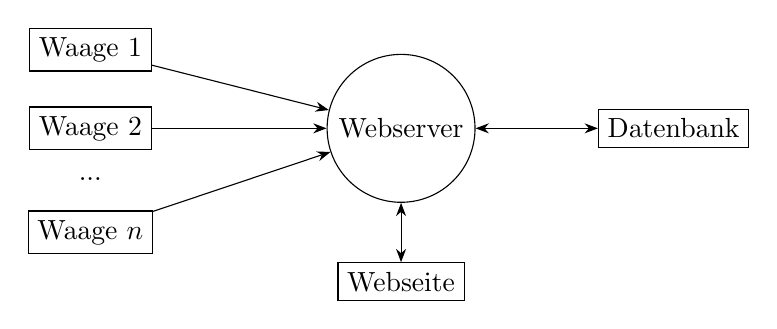
\begin{tikzpicture}

		\node[draw] (waage1) at (0,0) {Waage 1};
		\node[draw] (waage2) [below of = waage1] {Waage 2};
		\node[draw=none] (waage3) [below of = waage2, below = -0.5cm] {...};
		\node[draw] (waagen) [below of = waage3, below = -0.6cm] {Waage $n$};
		\node[draw, shape=circle] (server) [right of = waage2, right = 2cm] {Webserver};
		\node[draw] (app)    [below of = server, below = 0.7cm] {Webseite};
		\node[draw] (data)   [right of = server, right = 1.5cm] {Datenbank};

		\draw[-Stealth] (waage1) -- (server);
		\draw[-Stealth] (waage2) -- (server);
		\draw[-Stealth] (waagen) -- (server);
		\draw[Stealth-Stealth] (server) -- (data);
		\draw[Stealth-Stealth] (app) -- (server);
	\end{tikzpicture}
	\caption{Netzwerk Diagramm meines Serversystems\label{abb:networkdiagram}}
\end{figure}

Der Hauptbestanntteil meines Systems ist ein Zentraler Webserver welcher zur komonication mit der Webseite und den Bienenstockwaagen eine REST-API zur verfügung stellt.

% Die Waage {{{2
\subsection{Die Waage}

Die Bienenstockwaage funktioniert wie eine gewöhnliche Waage, welche man in dem meisten Haushalten findet.
Um zu verstehen, wie eine gewöhnliche Waage funktioniert muss man verstehen, wie eine Wägezelle funktioniert.

\begin{quote}
	\enquote{Wägezellen sind eine Sonderform der Kraftaufnehmer (Kraftsensoren) zum Aufbau von Wägevorrichtungen, d.h.\ zum Verwiegen mit Waagen.}~\cite[vgl.][]{WikiWaegezelle}
\end{quote}

\begin{wrapfigure}{l}{7cm}
	\centering
	\begin{circuitikz}[european]
		\draw (0, 4) to[battery1] (0,0) -- (3,0) to[R] (1,2) to[R] (3,4) to[R] (5,2) to[R] (3,0);
		\draw (0,4) -- (3,4);
		\draw (1,2) to[short, -*] (2,2) node[right]{$V_0$};
		\draw (5,2) to[short, -*] (4,2) node[left]{$V_1$};
	\end{circuitikz}
	\caption{Schaltung der Wägezellen\label{abb:circuit}}

\end{wrapfigure}

Sie besteht aus einem Federkörper\footnote{Metallstück welches etwas flexibel ist}, auf dem ein Dehnungsmessstreifen\footnote{Im folgenden als DMS abgekürzt} fixiert ist.
Dieser DMS verändert je nach Dehnung seinen elektrischen Widerstand.
Wegen dieser Eingenschaft bekommt man,
wenn man mehrere Wägezellen wie in Abbildung~\ref{abb:circuit} gezeigt verkabelt und den Spannungsunterschied zwischen $V_0$ und $V_1$ misst,
einen Spannungsunsterschied der in Relation zu dem Gewicht auf den Wägezellen ist.

Der Spannungsunterschied wird nun von einem Digital- zu A\-na\-log-Um\-wandler in ein digitales Signal umgewandelt welches mit Hilfe eines Mikrokontrolers weiter verarbeitet werden kann.
Bei einer gewöhnlichen Waage wird der Wert meist mit einer Konstante multipliziert damit der Wert einer Masseinheit($kg$) entspricht. Dieser wird auf einem Bildschirm dargestellt.

Im Falle meiner Waage wird der wird der Wert an den Server übermittelt.

% Kommunikation {{{2
\subsection[Kommunikation Waage --- Server --- DB]{Kommunikation Bienenstockwaage --- Server --- Datenbank}

% Initialisierung {{{3
\subsubsection[Initialisierung]{Initialisierung einer Bienenstockwaage}
Die Beinenstockwaagen schicken an den Server zum Initialisieren eine \texttt{GET} Anfrage an die URL \texttt{/init/<name>}, wo \texttt{<name>} durch den individuellen Namen der Waage ersetzt wird.
Der Server durchsucht darauf hin die Datenbank nach einem Dokument mit den Feld \texttt{name: <name>}.
Wenn er ein Dokument findet, schickt er die \texttt{\_id} des Dokuments an die Bienenstockwaage zurück.
Falls in der Datenbank jedoch kein Dokument mit dem Feld \texttt{name: <name>} enthalten ist,
erstellt er ein Dokument mit folgenden Feldern: \texttt{name: <name>} und \texttt{data: []}\footnote{\texttt{[]} ist die notation für ein leeres Array in vielen Programmiersprachen}. Siehe Listing~\ref{lst:document}
Anschließend sendet der Server die \texttt{\_id} des neu erstellten Dokuments zurück.
Sobald die Waage die Antwort des Servers bekommen hat speichert sie diese im Arbeitsspeicher.

\begin{listing}[H]
\begin{minted}[tabsize=2]{json}
{
	"_id": ObjectID,
	"name": "<name>",
	"data": [
		...,
		{
			"_id": ObjectID,
			"weight": 3505,
			"time": "2020-03-30T20:33:00.990+00:00"
		},
		...,
	]
}
\end{minted}
\caption{Dokument in Datenbank\label{lst:document}}
\end{listing}

% Datenübertagung {{{3
\subsubsection{Übertragung des Gewichts}
Zum Übertragen der Gewichtsdaten macht die Waage eine \texttt{POST} Anfrage an die URL \texttt{/add}, an die das aktuelle Gewicht des Bienenstockes und die bei der Initialisierung erhaltene DokementID im \texttt{JSON} Format angeheftet sind. Siehe Listing~\ref{lst:/add}.
\begin{listing}[ht]
\centering
\begin{minted}{http}
POST /add HTTP/1.1
User-Agent: PostmanRuntime/7.26.1
Host: www.beinenserver.com
Content-Type: application/json; charset=utf-8
Content-Length: <length>
Connection: Keep-Alive

{
	"_id": "5e8248aaf33b770d80370b68",
	"weight": 1000
}
\end{minted}
\caption{Beispiel einer \texttt{POST} Request auf \texttt{/add}}\label{lst:/add}
\end{listing}

Sobald der Server die Daten der Waage bekommen hat, holt er sich das Dokument mit der \texttt{\_id} aus der Anfrage aus der Datenbank und fügt ein neues Objekt mit dem Gewicht und der aktuellen Zeit (Listing~\ref{lst:objTimeWeight}) zum Dataarray des Dokumentes hinzu.
\begin{listing}[ht]
\centering
\begin{minted}{json}
{
	"time": "2020-03-30T20:33:00.990+00:00",
	"weight": 1000
}
\end{minted}
\caption{Objekt mit Zeit und Gewicht in \texttt{JSON}\label{lst:objTimeWeight}}
\end{listing}



% Literaturverzeichnis {{{1
\clearpage{}
\printbibliography{}
\end{document}
